\documentclass[preprint,12pt,a4paper]{elsarticle}

\usepackage{amssymb}
\usepackage{hyperref}
\usepackage{booktabs}
\usepackage{array}
\usepackage{graphicx}
\usepackage{float}
\setlength{\parindent}{0pt}

\journal{SoftwareX}

\begin{document}
\renewcommand{\labelenumii}{\arabic{enumi}.\arabic{enumii}}

% ---------------------------------------------------------------
\begin{frontmatter}

\title{EcoMarket: A Microservices-Based E-Commerce Platform for Ecological Products with AI-Driven Chemical Auditing}

\author[unal]{Josep Vladimir Garate Quispe\corref{cor1}}
\ead{josep.garate@est.unap.edu.pe}

\author[unal]{Arnold Diego Quispe Huanca}

\cortext[cor1]{Corresponding author.}

\address[unal]{Escuela Profesional de Ingeniería de Sistemas,
               Facultad de Ingeniería de Sistemas,
               Universidad Nacional del Altiplano,
               Puno, Peru}

% ---------------------------------------------------------------
\begin{abstract}
EcoMarket is a comprehensive e-commerce platform tailored for the Puno region in Peru, designed to connect local producers of ecological and organic products directly with environmentally conscious consumers. To combat the lack of verifiable organic certification and consumer distrust, the platform integrates an innovative Artificial Intelligence (AI) chemical auditing engine that analyzes product ingredients, assigns an ``Eco-Score'', and generates immutable PDF certificates with SHA-256 hashes. Built upon a robust microservices architecture, the system employs Next.js\,16 for the frontend, while the backend leverages a polyglot approach including Java (Spring Boot), Python (FastAPI), and Node.js (Express), interacting with PostgreSQL and MongoDB. The platform supports seamless local (Yape, Plin) and international (Stripe) payment methods, empowering rural agricultural producers by eliminating intermediaries.
\end{abstract}

\begin{keyword}
e-commerce \sep microservices \sep artificial intelligence \sep chemical auditing \sep Next.js \sep Spring Boot \sep FastAPI
\end{keyword}

\end{frontmatter}

% ---------------------------------------------------------------
% Información del Curso
% ---------------------------------------------------------------
\noindent\textbf{Curso:} Taller de Software \hfill \textbf{Docente:} Torres Cruz Fred

\vspace{0.5cm}

% ---------------------------------------------------------------
\section*{Required Metadata}

\section*{Current code version}

\begin{table}[!h]
\begin{tabular}{|l|p{5.8cm}|p{6.5cm}|}
\hline
\textbf{Nr.} & \textbf{Code metadata description} & \textbf{Please fill in this column} \\
\hline
C1 & Current code version & v1.0.0 \\
\hline
C2 & Permanent GitHub link to code/repository used for this code version &
     \url{https://github.com/JosepVl123463/EcoMarketFinalSoftware} \\
\hline
C3 & Legal Code License & MIT \\
\hline
C4 & Code versioning system used & git \\
\hline
C5 & Software code languages, tools, and services used &
     TypeScript, Next.js\,16, React, TailwindCSS, Java\,17, Spring Boot\,3.2, Python\,3.11, FastAPI, Node.js, Express, PostgreSQL, MongoDB, Docker \\
\hline
C6 & Compilation requirements, operating environments \& dependencies &
     Docker and Docker Compose for local orchestration. Backend services deployed on Render, frontend on Vercel. Databases on Neon (PostgreSQL) and MongoDB Atlas. \\
\hline
C7 & Link to developer documentation/manual &
     \url{https://eco-market-final-software-s2w6.vercel.app} \\
\hline
C8 & Support email for questions & josep.garate@est.unap.edu.pe \\
\hline
\end{tabular}
\caption{Code metadata (mandatory)}
\label{tab:code-metadata}
\end{table}

% ---------------------------------------------------------------
\section*{Current executable software version}

\begin{table}[!h]
\begin{tabular}{|l|p{5.8cm}|p{6.5cm}|}
\hline
\textbf{Nr.} & \textbf{Software metadata description} & \textbf{Please fill in this column} \\
\hline
S1 & Current software version & v1.0.0 \\
\hline
S2 & Permanent link to executables of this version &
     \url{https://eco-market-final-software-s2w6.vercel.app} \\
\hline
S3 & Legal Software License & MIT \\
\hline
S4 & Computing platform / Operating System & Any modern web browser
     (Chrome, Firefox, Safari, Edge); responsive design for mobile devices \\
\hline
S5 & Installation requirements \& dependencies & None for end-users.
     Developers: Docker, Node.js, Java, Python. \\
\hline
S6 & If available, link to user manual & \url{https://eco-market-final-software-s2w6.vercel.app} \\
\hline
S7 & Support email for questions & josep.garate@est.unap.edu.pe \\
\hline
\end{tabular}
\caption{Software metadata (mandatory)}
\label{tab:software-metadata}
\end{table}

% ---------------------------------------------------------------
\section{Motivation and Significance}

\subsection*{Context and Problem}

In the high-altitude region of Puno, Peru, traditional agriculture produces native, ecological crops such as quinoa, cañihua, and native potatoes. Despite this rich agricultural heritage, local smallholder producers face significant barriers to reaching broader markets, primarily relying on intermediaries that drastically reduce their profit margins (often by more than 70\%). 

Furthermore, consumers exhibit a growing demand for organic foods but lack a reliable mechanism to verify the authenticity of products claiming to be ecological. The absence of digital sales channels tailored for these producers, combined with a lack of integration with widely-used local payment methods (e.g., Yape, Plin), further hampers direct producer-to-consumer commerce.

\subsection*{Gap in Existing Solutions}

While general-purpose e-commerce platforms exist, they often lack specialized features required by the agricultural sector in developing regions, such as built-in chemical auditing, automated ecological scoring, and flexible payment gateways that encompass both international credit cards and localized mobile wallets. Currently, no solution offers an AI-driven verification system for product ingredients combined with immutable certification in the context of Andean agricultural products.

\subsection*{Contribution}

EcoMarket bridges this gap by providing an end-to-end digital commerce solution that ensures trust through an AI-powered chemical audit engine. The system evaluates product ingredients against databases of prohibited substances, calculates an ``Eco-Score'' (0--100), and issues verifiable PDF certificates secured with SHA-256 hashes. By facilitating direct sales through local payment networks and ensuring product quality, EcoMarket democratizes digital commerce for local producers.

% ---------------------------------------------------------------
\section{Software Description}

\subsection{Software Architecture}

EcoMarket employs a highly scalable microservices architecture. The application is divided into independent services that communicate via an API Gateway. The frontend, a Next.js\,16 Progressive Web App (PWA), is hosted on Vercel, while the backend microservices are containerized with Docker and deployed on Render.

\begin{figure}[!h]
\centering
\fbox{\parbox{0.85\textwidth}{\centering\vspace{1.2cm}
\textbf{[Insert Architecture Diagram]}\\
Frontend (Next.js) $\leftrightarrow$ API Gateway (Node.js) $\leftrightarrow$ Microservices (Auth, Product, Payment, Audit, AI, Notification) $\leftrightarrow$ Databases (PostgreSQL, MongoDB)\\
\vspace{1.2cm}}}
\caption{Microservices architecture of EcoMarket. An API Gateway routes traffic to specialized backend services, ensuring separation of concerns and independent scalability.}
\label{fig:arch}
\end{figure}

Key architectural highlights include:

\textbf{Polyglot Microservices:} Services are written in the most suitable language for their task: Java (Spring Boot) for core Auth and Product services, Python (FastAPI) for AI and Audit services, and Node.js for the API Gateway and Payment service.

\textbf{Hybrid Persistence:} A relational PostgreSQL database (hosted on Neon) manages structured data (users, products, orders), while a MongoDB Atlas document database stores flexible audit logs and ecological certificates.

\textbf{AI Audit Engine:} A dedicated Python service processes product ingredients, calculates the Eco-Score, and assigns badges (e.g., Eco-Friendly, Toxic-Free, Vegan) based on the analysis.

\textbf{Role-Based Access Control (RBAC):} A central Auth Service generates JSON Web Tokens (JWT) that define permissions across three roles: Client, Producer, and Administrator.

\subsection{Software Functionalities}

The platform supports distinct workflows tailored to its user roles:

\textbf{(a) Producer --- Catalog Management:} Producers register their agricultural products, providing descriptions, stock, pricing, and ingredient lists. Products initially hold a \texttt{PENDING} status, awaiting AI audit.

\textbf{(b) Administrator / AI System --- Chemical Auditing:} Administrators trigger the AI Audit Service for pending products. The system evaluates the ingredients, calculates the Eco-Score, assigns badges, and updates the product status to \texttt{APPROVED} ($\geq$70 score) or \texttt{RECHAZADO}. An immutable PDF certificate with a SHA-256 hash is generated.

\textbf{(c) Consumer --- Browsing and Purchase:} Consumers navigate a catalog filtered by category and minimum Eco-Score. They can view the audit certificates and add items to a cart managed globally by Zustand.

\textbf{(d) Consumer --- Checkout and Payments:} The checkout process integrates local Peruvian mobile payment systems (Yape, Plin) as well as Stripe for international credit cards, updating inventory in real time.

\subsection{Database Schema and Domain Models}

The data architecture is distributed across the microservices. The core relational models include:

\begin{table}[!h]
\centering
\begin{tabular}{lp{9.5cm}}
\toprule
\textbf{Entity} & \textbf{Description} \\
\midrule
\texttt{User}            & Core identity data (Name, Email, Password Hash, Role). \\
\texttt{ProducerProfile} & Extension of User for producers (RUC, certifications, GPS origin). \\
\texttt{Product}         & Catalog item with status (PENDING, APPROVED, REJECTED), ingredients, and stock. \\
\texttt{Order}           & E-commerce transaction linking User, Products, and Payment Status. \\
\texttt{AuditRecord}     & (MongoDB) Stores the AI evaluation results, Eco-Score, and SHA-256 hash. \\
\bottomrule
\end{tabular}
\caption{Primary domain entities across the microservices.}
\label{tab:schema}
\end{table}

% ---------------------------------------------------------------
\section{Illustrative Examples}

In practice, a producer in Puno can log in, upload a batch of native quinoa, and submit it for review. The AI engine processes the entry, confirms the absence of prohibited agrochemicals, and assigns an Eco-Score of 95 along with a `Toxic-Free` badge. When a consumer views the platform, they see the verified quinoa, complete with the downloadable SHA-256 signed audit certificate. The consumer adds the product to their cart and pays seamlessly using Yape. A push notification is instantly sent to the producer to fulfill the order.

The following figures show the main screens of the deployed EcoMarket platform.

% --- Figura 1: Página de Inicio ---
\begin{figure}[H]
\centering
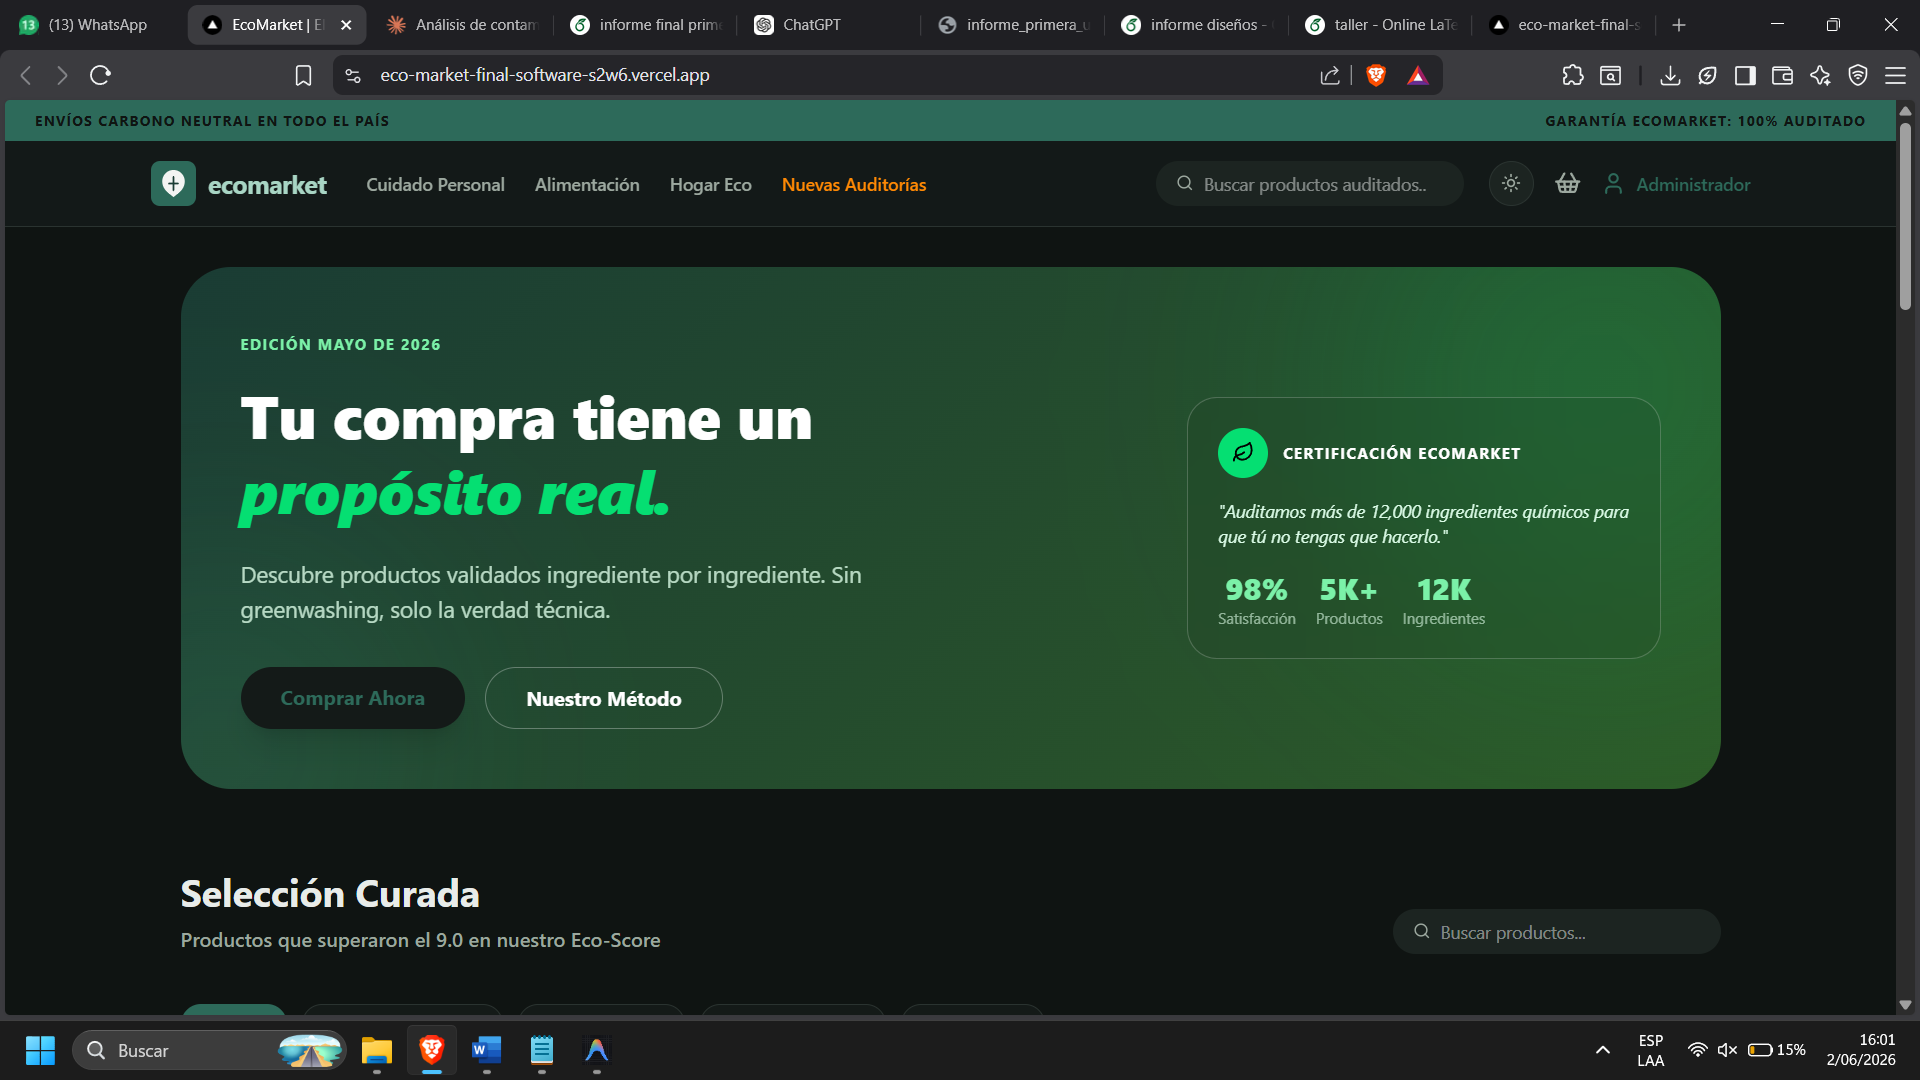
\includegraphics[width=0.95\textwidth]{images/home.png}
\caption{EcoMarket home page. The main banner highlights the platform's value proposition: AI-audited products with no greenwashing. Key metrics (98\% satisfaction, 5K+ products, 12K audited ingredients) are prominently displayed.}
\label{fig:home}
\end{figure}

% --- Figura 2: Catálogo de Productos ---
\begin{figure}[H]
\centering
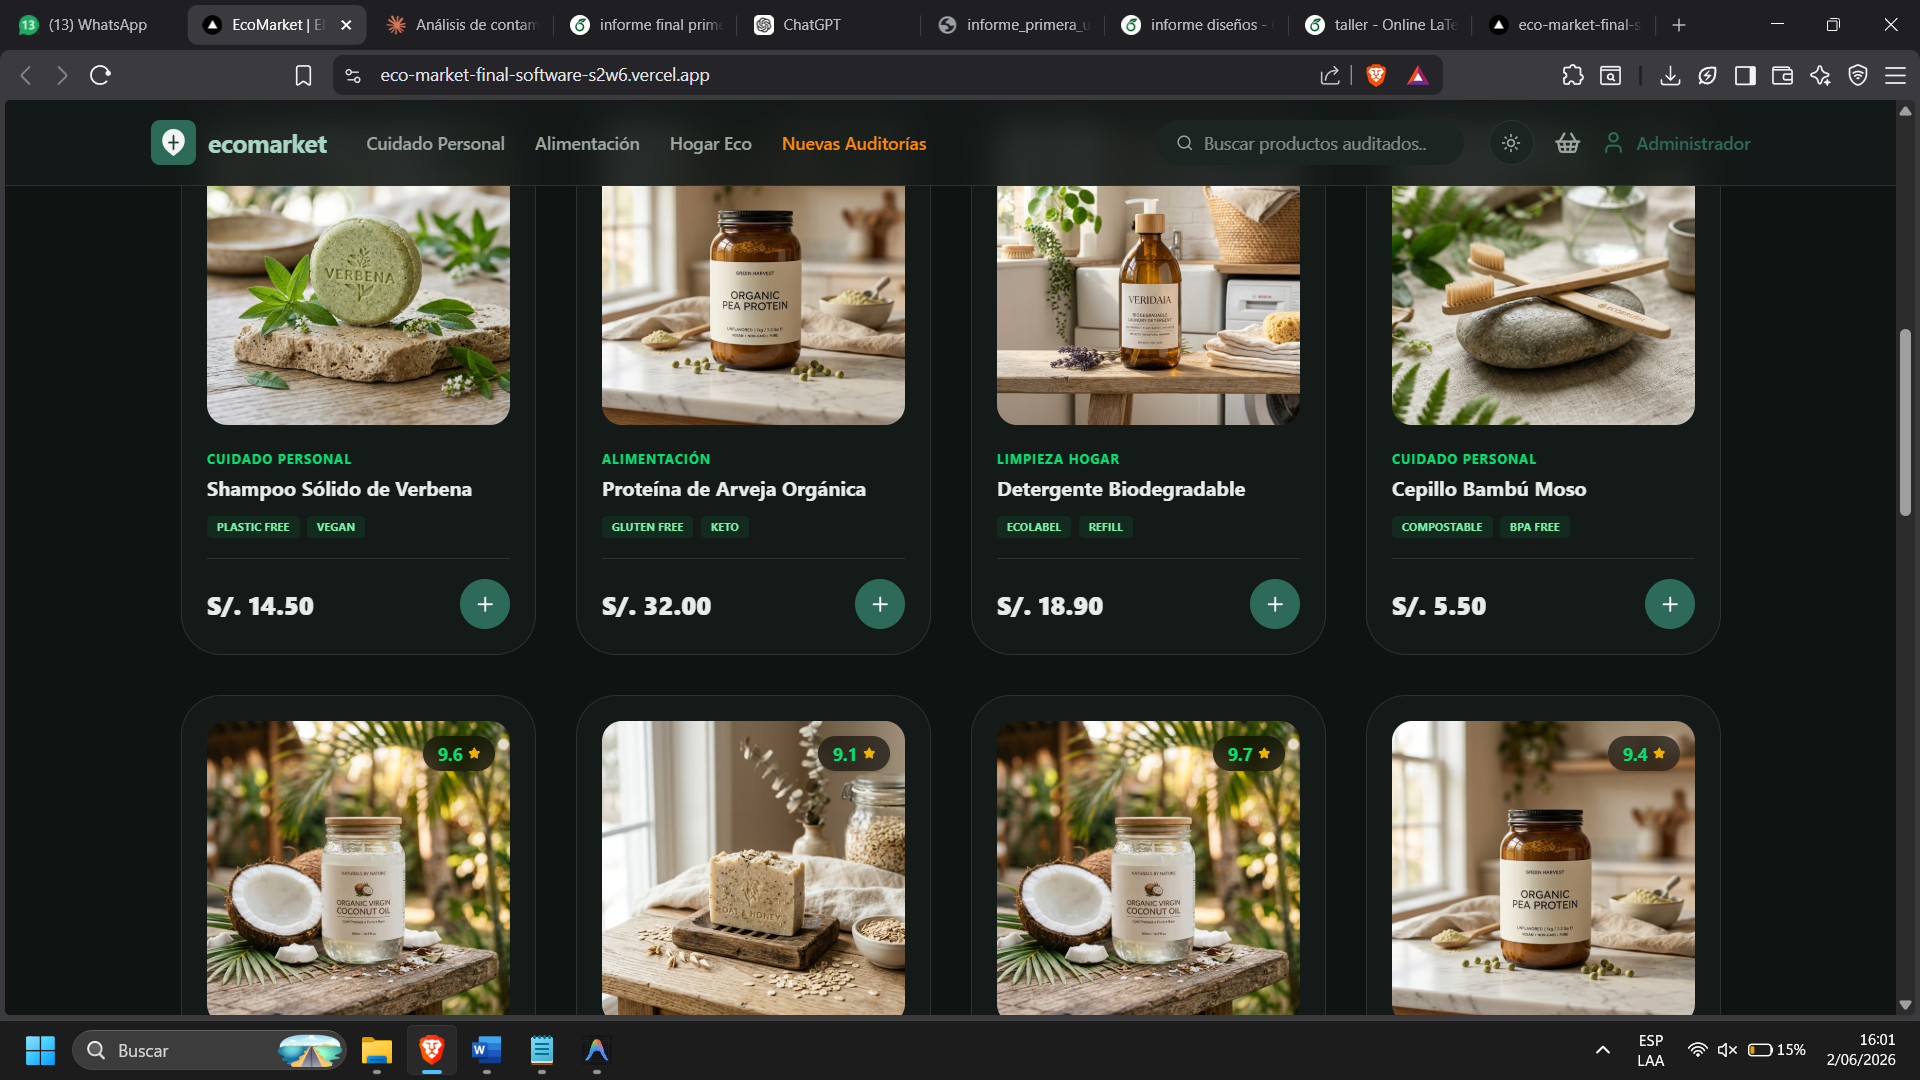
\includegraphics[width=0.95\textwidth]{images/catalogo.png}
\caption{Product catalog showing ecological items (e.g., Shampoo Sólido de Verbena, Proteína de Arveja Orgánica) along with their ecological badges (PLASTIC FREE, VEGAN, GLUTEN FREE, KETO) and Eco-Score ratings assigned by the AI audit engine.}
\label{fig:catalogo}
\end{figure}

% --- Figura 3: Panel Administrativo ---
\begin{figure}[H]
\centering
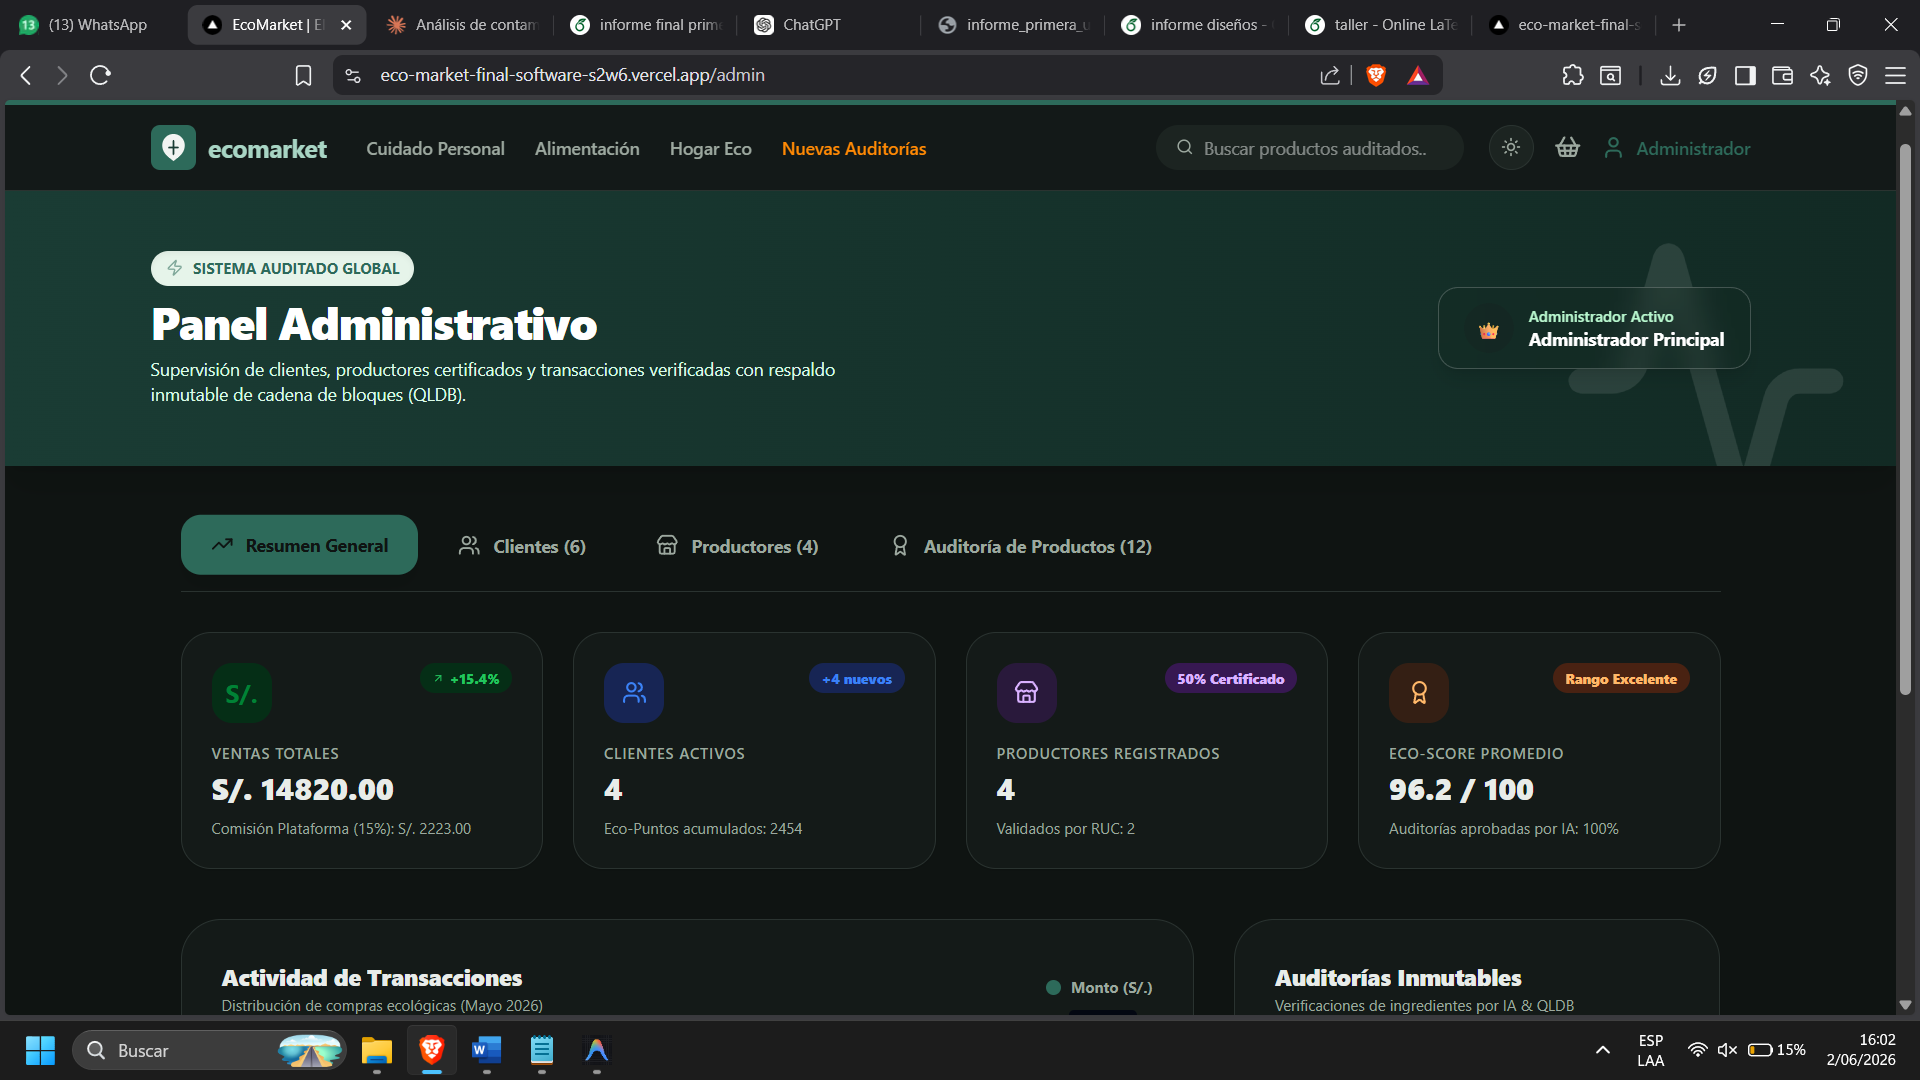
\includegraphics[width=0.95\textwidth]{images/admin.png}
\caption{Administrative dashboard displaying real-time KPIs: total sales (S/. 14,820), active clients (4), registered producers (4), and an average Eco-Score of 96.2/100 with 100\% AI-approved audits. The panel also lists immutable audit records backed by QLDB blockchain technology.}
\label{fig:admin}
\end{figure}

% --- Figura 4: Inicio de Sesión ---
\begin{figure}[H]
\centering
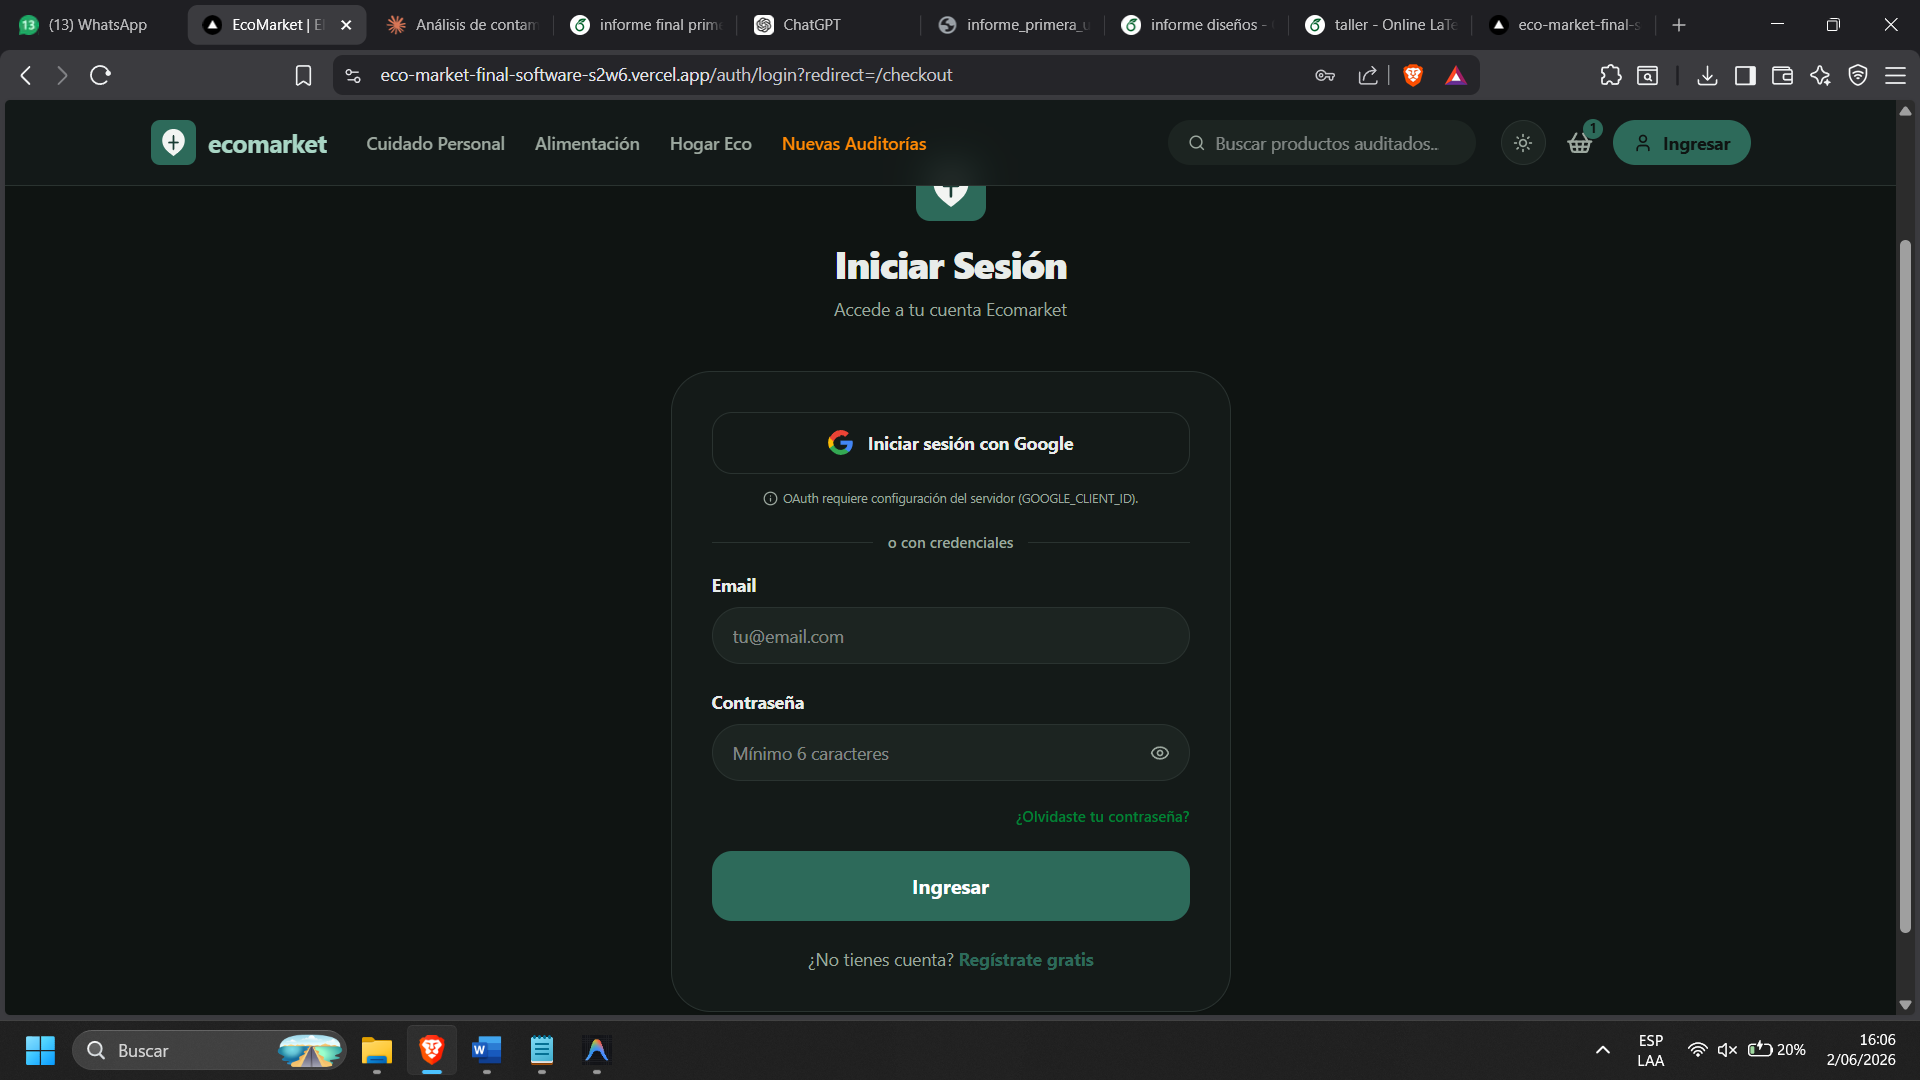
\includegraphics[width=0.85\textwidth]{images/login.png}
\caption{Authentication screen supporting Google OAuth and credential-based login (email and password), providing secure role-based access for clients, producers, and administrators.}
\label{fig:login}
\end{figure}

% --- Figura 5: Pago con Yape ---
\begin{figure}[H]
\centering
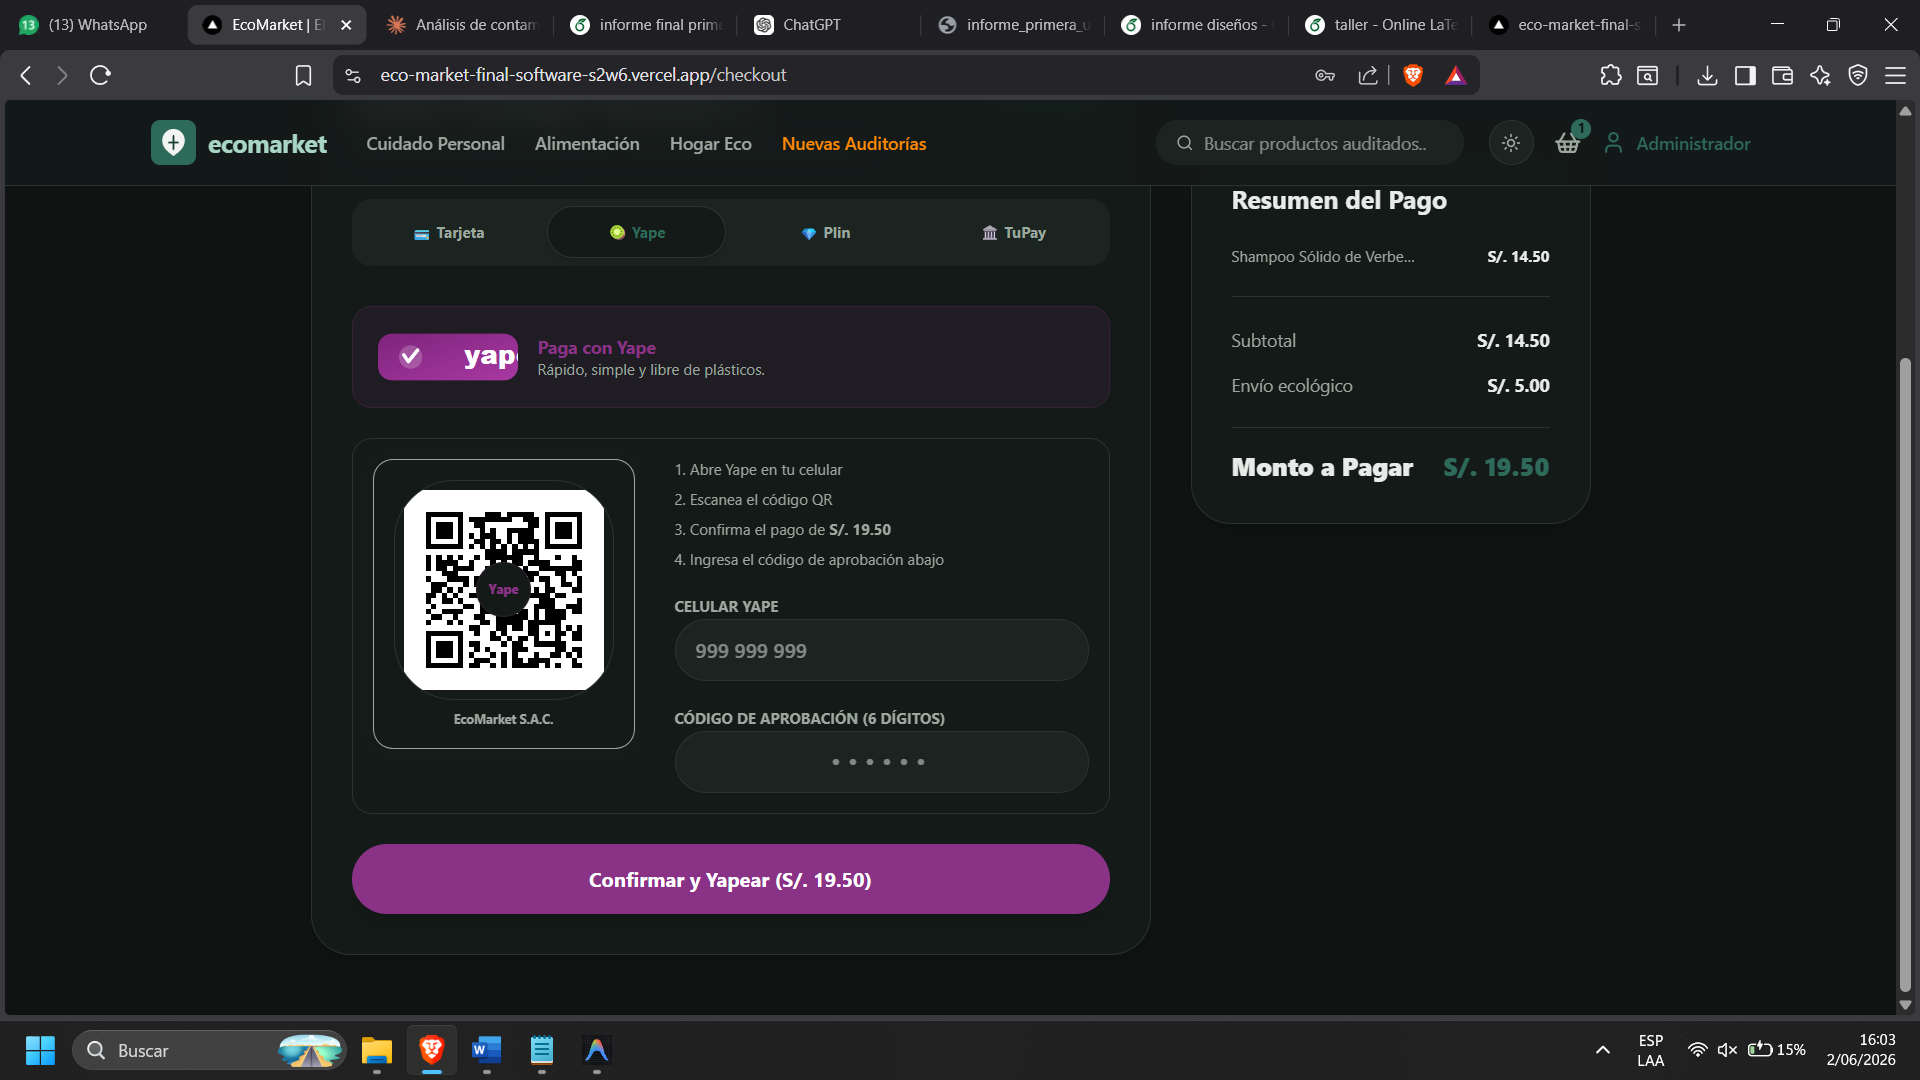
\includegraphics[width=0.85\textwidth]{images/checkout_yape.png}
\caption{Checkout screen with Yape payment integration. The user scans a dynamic QR code generated for the transaction amount (S/. 19.50) and enters a six-digit approval code. The payment summary confirms the selected product and ecological shipping fee.}
\label{fig:checkout}
\end{figure}

% ---------------------------------------------------------------
\section{Impact}

\subsection*{Empowering Local Producers}
EcoMarket directly tackles the issue of low profit margins for farmers by providing a direct-to-consumer channel. The integration of zero-barrier payment methods like Yape ensures that rural producers without traditional bank accounts can participate in digital commerce.

\subsection*{Fostering Consumer Trust}
The AI-driven chemical auditing system replaces subjective claims of ``organic'' with quantifiable, verifiable metrics. The generation of immutable PDF certificates guarantees transparency and builds trust, which is critical for scaling e-commerce for ecological goods.

\subsection*{Educational and Research Value}
Developed as part of the \textit{Taller de Software} course under the guidance of Professor Torres Cruz Fred at the Universidad Nacional del Altiplano (Puno), EcoMarket serves as a comprehensive case study in microservices design, polyglot persistence, AI integration, and secure JWT-based authentication. The codebase provides a blueprint for building scalable, cloud-native SaaS applications in academic environments.

% ---------------------------------------------------------------
\section{Conclusions}

EcoMarket demonstrates how modern cloud-native architectures and Artificial Intelligence can be combined to solve real-world socio-economic problems in the agricultural sector. By offering an automated chemical auditing system alongside localized e-commerce functionalities, the platform empowers producers in Puno, Peru, and ensures product quality for consumers. The microservices architecture provides a scalable, maintainable foundation that can be adapted for similar ecological markets worldwide.

% ---------------------------------------------------------------
\section*{Acknowledgements}

The authors acknowledge the Consorcio de Ingeniería de Software and the faculty of the Universidad Nacional del Altiplano, Puno, for their guidance during the development of this project. Special thanks to Professor Torres Cruz Fred, instructor of the \textit{Taller de Software} course, for his mentorship throughout this project. The authors also thank the agricultural producers and consumers who provided valuable feedback during the requirements gathering phase.

\end{document}
